\chapter{Umsetzung}

Umgesetzt wurde die Aufgabe im wesentlichen aus drei Teilen: 
\begin{itemize}
	\item Einer SQL-Datenbank mit realitätsnahen Tabellen 
	\item Einer Ontologie 
	\item Einem ausführbaren Programm mit Grafischer Benutzungsoberfläche

\end{itemize}

\section{Datenbank}

Bei der Datenbank wurde auf eine gewöhnliche relationale Datenbank zurückgegriffen, da im wesentlichen nur die gängigsten SQL-Befehle benutzt werden. Da es bereits gute Erfahrungen im Team mit MySQL gab, wurde diese Datenbank verwendet. 

Die Datenbank enthält im wesentlichen Informationen die ein Hochschulsportberater ebenfalls nachschlagen würde. Die wichtigsten Informationen sind:
\begin{itemize}
\item angebotene Sportarten
\item Trainingszeiten
\item Veranstaltungsort
\item Höhe der Teilnehmergebühr
\end{itemize} 
Das genaue Datenbankmodell kann der Abbildung \ref{fig:Datenbank-Design} entnommen werden.

\begin{capfigure}[Datenbank-Design]
	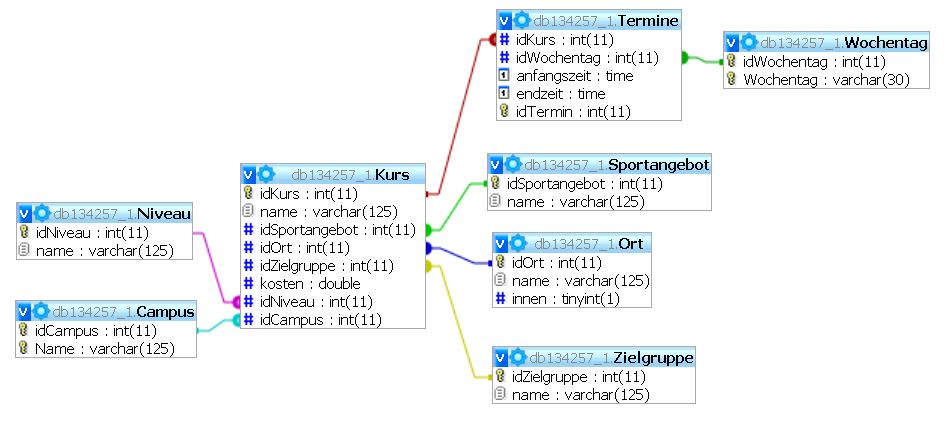
\includegraphics[width=\textwidth]{images/db_design}
\end{capfigure}

\section{Ontologie}
\TODO{[PRIO:SOFORT] Komplett neu machen}
Die Erstellung der Ontologie wird mit \gls{protege} durchgeführt. \gls{protege} ermöglicht nur die Verwendung von OWL-DL. OWL-Full wird nicht unterstützt, daher müssen gewisse Einschränkungen berücksichtigt werden. Beispielsweise kann man keine Komplementklassen erstellen. 

Des Weiteren sollte man immer bedenken, dass eine Ontologie ein Open-World-Szenario darstellt. Im Speziellen kann man nur nach dem Vorhandensein eines Kriteriums abfragen.

Im Laufe dieses Abschnitts wird erläutert, wie die Ontologie erstellt wurde. Im Besonderen werden unsere Entscheidungen bei der Umsetzung begründet und deren Folgen erklärt.

\subsection{Grobe Unterteilung der Ontologie}
Zuerst wird die Klasse \textit{Sport} erstellt. Diese Klasse enthält die beiden Unterklassen \textit{Einzelsport} und \textit{Teamsport}. Da wir uns bei den Sportarten dafür entschieden haben, dass eine Sportart entweder Einzelsport oder Teamsport ist macht diese Unterteilung am meisten Sinn. Natürlich ermöglicht diese Lösung nicht, dass eine Sportart zugleich Einzelsport als auch Teamsport ist. Dies ist aber kein Problem, da es in unserem Szenario nicht vorkommt.

Bei der Darstellung der Ontologie lassen wir die Ebene \textit{Thing} aus Gründen der Übersichtlichkeit weg.
Die Ontologie sieht jetzt wie folgt aus:
\begin{capitemize}[Ontologie - Grober Unterteilung der Ontologie - 1]
		\item Sport
			\begin{itemize}
				\item Einzelsport
				\item Teamsport
			\end{itemize}
\end{capitemize}

Als Nächstes legen wir die Klassen \textit{Ziele} und \textit{Koerperliche\_Einschraenkungen} an. Diese beiden Klassen dienen dazu, die Eigenschaften \textit{Ziele} und \textit{Koerperliche\_Einschraenkungen} abzubilden. Beide Klassen werden noch mit den jeweiligen Unterklassen, die die möglichen Optionen darstellen ergänzt.

Danach sieht die Ontologie wie folgt aus:
\begin{capitemize}[Ontologie - Grober Unterteilung der Ontologie - 2]
	\item Koerperliche\_Einschraenkungen
		\begin{itemize}
				\item Armbereich
				\item Beinbereich
				\item Hoehenangst
		\end{itemize}
	\item Sport
		\begin{itemize}
			\item Einzelsport
			\item Teamsport
		\end{itemize}
	\item Ziele
		\begin{itemize}
				\item Fitness
				\item Freizeitvergnuegen
				\item SelfDefense
				\item Sozialkontakte
				\item Wettbewerb
		\end{itemize}
\end{capitemize}

Damit sind die Klassen soweit fertig. Beide Klassen wurden in dieser Art angelegt, da sie optional sind. Ein Sport muss keine Verknüpfung zu diesen Klassen haben. \TODO{Ich versteh was du meinst, aber erst beim 2ten Lesen. Bitte umformulieren.} Jetzt werden noch die Object Properties dazu wie folgt angelegt: 

\begin{capitemize}[Properties - hatZiel und ungeeignetBei]
	\item hatZiel
		\begin{itemize}
			\item Domains: \textit{Sport}
			\item Ranges: \textit{Ziele}
		\end{itemize}
	\item ungeeignetBei
		\begin{itemize}
			\item Domains: \textit{Sport}
			\item Ranges: \textit{Koerperliche\_Einschraenkungen}
		\end{itemize}
\end{capitemize}

Nun lassen sich die Ziele und Einschränkungen mit den Sportarten verbinden. Ein Problem ergibt sich mit dieser Variante allerdings noch, man kann nicht nach Sportarten suchen die explizit keine Einschränkungen haben. Bei den Zielen gibt es die gleiche Einschränkung \TODO{Das Wort Einschränkung hat eine doppelte Bedeutung. Bitte anderes Wort benutzen, oder immer körperliche Einschränkung verwenden}, allerdings ist sie dort egal, da eine Suche nach Sportarten, die explizit keine Ziele haben keinen Sinn ergibt. Bei den Einschränkungen muss allerdings eine Lösung her. Da in einem Open-World-Szenario nur nach dem Vorhandensein gefragt werden kann, haben wir uns dazu entschieden noch die Unterklasse \textit{Keine} bei den Körperlichen Einschränkungen zu ergänzen. Jetzt hat man die Möglichkeit, auch Sportarten zu suchen, die bei keiner Einschränkung ungeeignet sind.

Bei den Sportarten muss jetzt jede Sportart die Object Property \textit{ungeeignetBei} verwenden.  \TODO{Bitte noch erwähnen, dass Keine explizit gesetzt werden muss.} Für die Object Property \textit{hatZiel} gilt das nicht. \TODO{Warum? Bitte in einem Satz erläutern.}

\TODO{Erläutern was die folgende Liste darstellt.}
\begin{capitemize}[Properties - istExotisch, istKampfsport, istKoerperkontakt, istWassersport]
	\item istExotisch
		\begin{itemize}
			\item Domains: \textit{Sport}
			\item Ranges: \textit{Boolean}
		\end{itemize}
	\item istKampfsport
		\begin{itemize}
			\item Domains: \textit{Sport}
			\item Ranges: \textit{Boolean}
		\end{itemize}
	\item istKoerperkontakt
		\begin{itemize}
			\item Domains: \textit{Sport}
			\item Ranges: \textit{Boolean}
		\end{itemize}
	\item istWassersport
		\begin{itemize}
			\item Domains: \textit{Sport}
			\item Ranges: \textit{Boolean}
		\end{itemize}
\end{capitemize}

Alternativ wäre eine Realisierung über Data-Properties möglich gewesen (mit dem eingebauten Typ boolean als Range). Für die Einführung einer eigenen Klasse Boolean wurde mit den Unterklassen "`True"' und "`False"' als Range für die Object Properties haben wir uns entschieden, da es von der Komplexität her gleichwertig war. Außerdem ist dies übersichtlicher. Der Restriktionstyp "`value"' ist außerdem beim den Restriktionseditoren von Protégé beim Anlegen von Äquivalenzklassen nicht in der Dropdownbox aufgetaucht, so dass die Lösung über Object-Properties unterm Strich vereinfacht hat.
\TODO{Satzbau, Kontext. Ich versteh nicht auf was du hinauswillst.}

\TODO{istExotisch, istKampfsport, istKoerperkontakt, istWassersport - Problem erw\"ahnen, dass man nicht nach Boolean abfragen kann}

\subsection{Äquivalenzklassen}

Um die Ontologieprobleme in den Szenarien zu lösen, wurden in der Ontologie bereits Äquivalenzklassen beschrieben. Folgende Äquivalenzklassen wurden eingeführt:

\TODO{format + Erläutern}
\TODO{Äquivalenzklassen nur kurz erwähnen. Auf keinen Fall alle aufzählen. Diese werden im Programm kaum benutzt. Die einzige die mir gerade einfällt ist Koerperliche\_Einschraenkungen, da man durch diese die tatsächlichen Einschränkungen abbilden kann.}

\textbf{Sport}
ExotischeSportarten  
	istExotisch only True
	
FitnessZiel
	hatZiel some Fitness
	
FreizeitvergnuegenZiel
	hatZiel some  Freizeitvergnuegen)
	
GeeignetBeiArmbereichKE
	Sport and (not (ungeeignetBei Armbereich))
	
GeeignetBeiBeinbereichKE
	Sport and (not (ungeeignetBei some Beinbereich))
	
GeeignetBeiHoehenangst
	Sport and (not (ungeeignetBei some Hoehenangst))
	
Kampfsportarten 
	Sport and (istKampfsport only True)
	
Koerperkontaktsportarten 
	Sport and (istKoerperkontakt only True)
	
NichtexotischeSportarten 
	Sport and (istExotisch only False)
	
Nichtkampfsportarten 
	Sport and (istKampfsport only False)
	
NichtkoerperkontaktSportarten 
	Sport and (istKoerperkontakt only False)
	
Nichtwassersportarten 
	Sport and (istWassersport only False)
	
SelfDefenseZiel 
	hatZiel some SelfDefense
	
SozialkontakteZiel 
	hatZiel some Sozialkontakte
	
Wassersportarten 
	Sport and (istWassersport only True)
	
WettbewerbZiel 
	hatZiel some Wettbewerb
	
\textbf{Koerperliche\_Einschraenkungen}
Koerperliche Einschränkung
Armbereich
 or Beinbereich
 or Hoehenangst

\TODO{\"Aquivalenzklassen, Aufbau einer Sportart, etc. - ausformulieren}

\TODO{Ich habe die Ontologie ja nachträglich noch erweitert. Es ist jetzt die Frage, wie wir diese Änderungen rein nehmen. Meiner Meinung ist es das Beste, wenn du die Personen und neuen Properties kurz erwähnst und dann auf das entsprechende Kapitel oder Abschnitt verweist. das müsste mit \textbackslash nameref gut gehen. }

\section{Programm}

Dieser Abschnitt geht zuerst auf die Entscheidung zum Aufbau der graphischen Oberfläche ein und behandelt danach die technischen Aspekte des Programms. 

\subsection{Entscheidung zum Aufbau der graphischen Oberfläche}
Bei der Gestaltung der GUI, wurde sich dafür entschieden, dass der Benutzer zu jedem Zeitpunkt möglichst alle Auswahlmöglichkeiten vor Augen hat und dass er, ebenfalls zu jedem Zeitpunkt, eine Liste mit den Sportarten erhalten kann, die zu seinen Auswahlkriterien passen.

Die Gründe für diese Entscheidungen sind zum einen die Benutzerfreundlichkeit. Durch diesen Aufbau soll der Benutzer aufgefordert werden, möglichst viele Auswahlkriterien auszuprobieren, da er sofort testen kann, welche Auswirkungen diese auf die Auswahl der Sportarten hat. Dies hat den Vorteil, dass der Benutzer die Kriterien mit, einer für ihn, hohen Priorität setzen kann und unangerührt lässt, währendem er die Kriterien mit einer, für ihn, niedrigen Priorität schnell und einfach ändern kann. Ein konkretes Beispiel hierfür wäre z.B. die Sportart Klettern. Für einige Benutzer ist die Höhenangst nur ein leichtes Problem, für einige andere ist sie unüberwindlich. Somit haben die Benutzer mit leichter Höhenangst, die Möglichkeit die angebotenen Sportarten mit oder ohne Höhenangst zu vergleichen, während jene mit starker Höhenangst das Kriterium auswählen und nicht mehr deaktivieren.

Ein anderer Grund für diese Entscheidung war die Tatsache, dass unsere Szenarien wenige Sprünge von einem Schritt zu einem anderen beinhalten. Deshalb haben wir uns dagegen entschieden eine Frage nach der anderen abzuhandeln, wie die Szenarien dies eigentlich vorsehen und bei mehreren Sprüngen wohl auch einfacher umzusetzen gewesen wäre. Nichtsdestotrotz wird am Ende dieses Abschnittes erläutert wie mehrere dieser Sprünge dargestellt werden könnten, obwohl der Benutzer nach wie vor sämtliche Optionen vor Augen hat und möglichst wenig an Flexibilität einbüßt.
\TODO{richtige referenz setzen}

\subsection{Aufbau der graphischen Oberfläche}

Bei der Abbildung \ref{fig:Hauptfenster} handelt es sich um das Hauptfenster, in dem der Benutzer die Möglichkeit hat seine Auswahlkriterien festzulegen, die Suche zu starten sowie die vorgeschlagen Sportarten einzusehen und Informationen über diese zu erhalten. Bei den Auswahlkriterien handelt es sich um jene, die benötigt werden, um die Fragen aus den Szenarien zu beantworten.

Bei der Abbildung \ref{fig:Auswahl der Zeiten} handelt es sich um einen "`Stundenplan"', in dem der Benutzer die Zeiträume festlegen kann, in denen er wöchentlich Sport treiben will. 

%\begin{capfigure}[Hauptfenster]%
%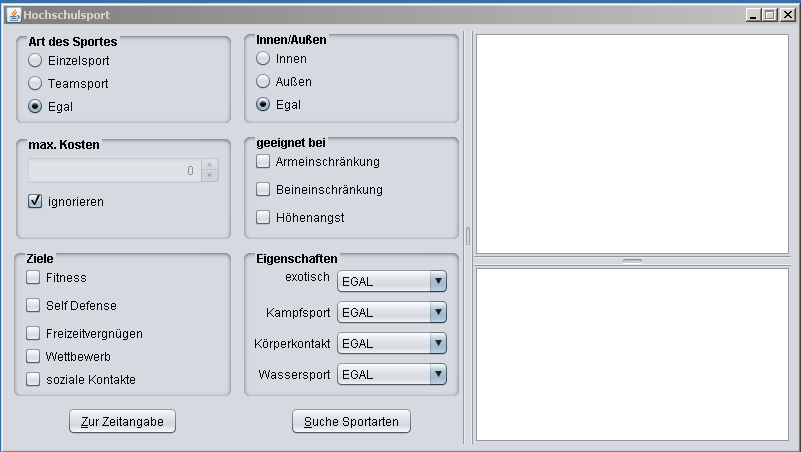
\includegraphics[width=\textwidth]{images/gui.png}%
%\end{capfigure}

%\begin{capfigure}[Auswahl der Zeiten]%
%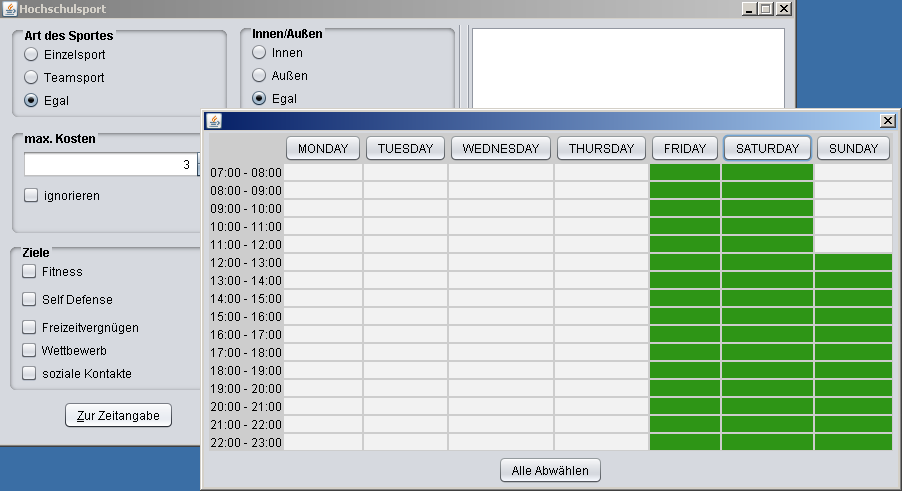
\includegraphics[width=\textwidth]{images/guizeit.png}%
%\end{capfigure}

\begin{figure}[p]
\centering
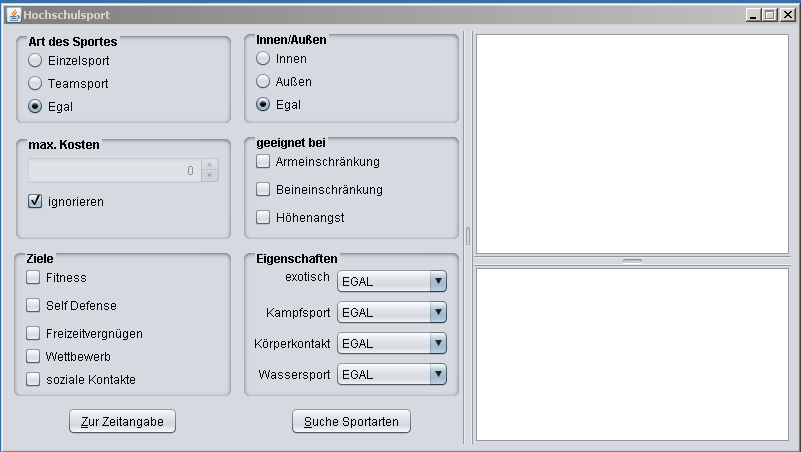
\includegraphics[width=\textwidth]{images/gui.png}%
\caption{Hauptfenster}
\label{fig:Hauptfenster}
\end{figure}

\begin{figure}[p]
\centering
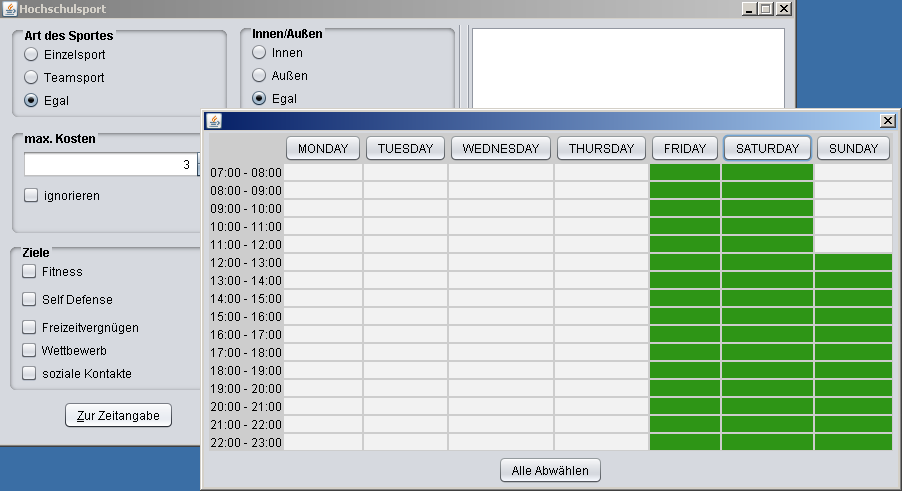
\includegraphics[width=\textwidth]{images/guizeit.png}%
\caption{Auswahl der Zeiten}
\label{fig:Auswahl der Zeiten}
\end{figure}
\newpage
\subsection{Technische Umsetzung}
Das Programm wurde mit Java geschrieben und benutzt die Semantic Web OWL API \autocite{semweb:owlapi} als Verbindung zur Ontologie. Beim benutzten Reasoner handelt es sich um HermIT\autocite{krr:hermit}. Die Verbindung zur Datenbank wird durch einen JDBC-Treiber\autocite{oracle:jdbc} realisiert.

Beim Ausführen der Suche wird zunächst eine Menge mit sämtlichen verfügbaren Sportarten erstellt, die daraufhin nach Bedarf gefiltert wird. Der Einfachheit halber wird für jedes Auswahlkriterium, falls dieses nicht ignoriert werden soll, eine Query ausgeführt, die die Menge mit den Sportarten weiter filtert. Jede Query hat folgenden, gleichen Aufbau\footnote{UML angelehnte Schreibweise \lstinline"  operation(arg list) : return type" \autocite{kow:umlclass}} \lstinline"query(Sportarten) : gefilterte_Sportarten". Dies bedeutet, dass eine Query eine Menge von Sportarten enthält und nach einem bestimmten Auswahlkriterium filtert, um dann die gefilterte Menge zurückzugeben. Durch den jeweils gleichen Aufbau ergibt sich der Vorteil, dass die Reihenfolge der Queries keine Rolle spielt, und sie demnach auch bei Bedarf übersprungen werden können. Das Überspringen von Queries wird benötigt, da jedes Auswahlkriterium vom Benutzer ignoriert werden kann und somit keinen Einfluss auf den Auswahlprozess nimmt.

Das Listing \ref{lst:filtern} zeigt das Filtern an einem konkreten Beispiel. In einem ersten Schritt werden die Sportarten abgefragt. Danach werden die einzelnen Queries durchlaufen, wobei immer abgefragt wird, ob das entsprechende Auswahlkriterium nicht ignoriert werden soll. Im Beispiel wird der nach dem maximalen Preis und den Zielen gefiltert. Es sei noch darauf hingewiesen, dass es an dieser Stelle im Code keinen Unterschied macht, ob die Query über die Datenbank (für den Preis) oder die Ontologie (für die Ziele) ausgeführt wird. 

\begin{lstlisting}[float=htbp, caption=Filtern von Sportarten, label=lst:filtern]
Set<Sportangebot> sport = Queries.querySport();
...        
if (!ignorePrice) {
	sport = Queries.queryPrice(sport, maximalPrice);
}
...
if (ziele.length > 0) {
	//der Benutzer hat Ziele ausgewaehlt
	sport = Queries.queryZiele(sport, ziele);
}
...                
\end{lstlisting}